\documentclass[../Languages.tex]{subfiles}

\begin{document}
\usec{Java}\label{sec:java}

\cd{Java} is a general-purpose computer programming language that is
concurrent, class-based, object oriented, and specifically designed to have as
few implementation dependencies as possible. It is intended to let application
developers ``write once, run anywhere'' (WORA), meaning that compiled
\cd{Java} code can run on all platforms that support \cd{Java} without
the need for recompilation. \cd{Java} applications are typically compiled
to byte code that can run on any \textit{Java virtual machine} (JVM) regardless
of computer architecture. As of 2016, \cd{Java} is one of the most popular
programming languages in use, particularly for client-server web applications,
with a reported 9 million developers. \cd{Java} was originally developed by
James Gosling at Sum Microsystems (which has since been acquired by Oracle
Corporation) and released in 1995 as a core component of Sum Microsystems' Java
platform. The languages derives much of its syntax from \cd{C} and
\cd{C++}, but it has fewer low-level facilities than either of them.

The original and reference implementation \cd{Java} compilers, virtual
machines, and class libraries were originally released by Sun under proprietary
licenses. As of May 2007, in compliance with the specifications of the Java
Community Process, Sum relicensed most of its \cd{Java} technologies under
the GNU General Public License. Others have also developed alternative
implementations of these Sun technologies, such as the GNU Compiler for
\cd{Java} (byte code compiler), GNU ClassPath (standard libraries), and
IcedTea-Web (browser plugin for applets).

The latest version is \cd{Java 9}, released on September 21, 2017, and is
one of the two version currently supported for free by Oracle. Versions earlier
than \cd{Java 8} are supported by companies on a commercial basis; e.g. by
Oracle back to \cd{Java 6} as of October 2017.

\subsection{Influence}\label{sub:influence}

\begin{Figure}
  \centering
  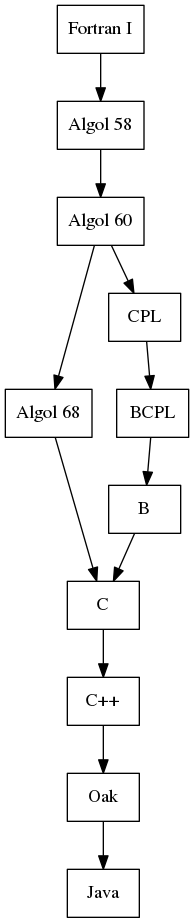
\includegraphics[height=0.5\textheight]{java}
  \captionof{figure}{Inheritance diagram for \cd{Java}.}
\end{Figure}

\newpage
\end{document}
